\documentclass{article}

\usepackage{graphicx}
\usepackage[utf8]{inputenc}

\title{Exabiome Journal}
\author{ajtritt }
\date{April 2020}

\begin{document}

\maketitle

\section{Introduction}

\subsubsection*{Wed Apr 22, 2020}

I trained the RozNet network (i.e. AlexNet, adjusted for one-hot-encoded DNA sequences) to predict taxonomy
from 11-dimensional UMAP embeddings (i.e. regression problem) and just class labels (i.e. classification problem).

I tried different dropout rates, removing batch norm at the last layer, using max pooling instead of average pooling
between convolution and fully-connected layers, adding more FC layers, and changing convolution stride. None of these
things appear to impact network performance. I suspect that the model is too complex, and is overfitting the data. I
think this because the test performance never improves and is significantly worse than the train performance. See
Figure~\ref{fig:roznet_train_test}.

\subsubsection*{Thu Apr 23, 2020}
Earlier, I also ran a simple neural network (1 Conv layer, 3 fc layers). Train loss bottomed out around 53 MSE, similar
to what previous networks were achieving. This was after about 35 epochs, before it crashed because sequences a bad
batch could not be passed through the network. This led to me looking into why this problem kept happening, and I discovered
that my sequence storage mechanism of packing bits was not being read correctly. I think this might be why I networks are
not training.


\begin{figure}
  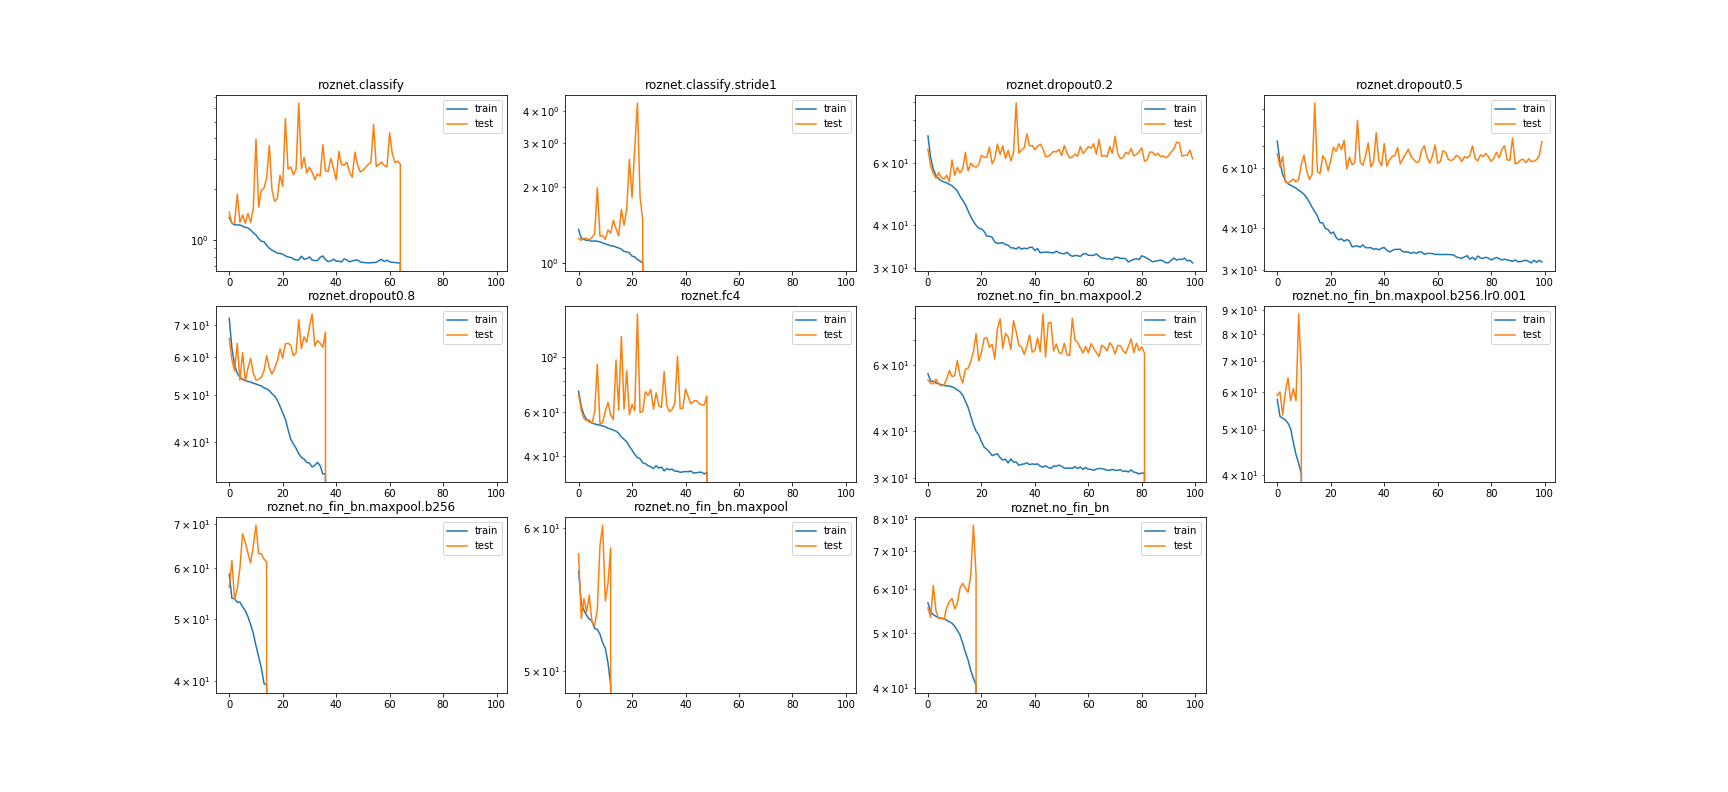
\includegraphics[width=\linewidth]{roznet_results.png}
  \caption{Train and test loss results for RozNet}
  \label{fig:roznet_train_test}
\end{figure}

\subsubsection*{Thu May 28, 2020}
I reformatted the data to store label-encoded DNA (i.e. integer encoding) using the HDMF VocabData column type. I ran
a few different networks/problems, and it appears that training is working (See Figure~\ref{fig:encoding_fix_results}. Now I am having issues with running out of
memory. I have reworked my training code to use PyTorch-Lightning to handle running on GPUs etc. I will try that, and
also explore using 16-bits for training.

\begin{figure}
  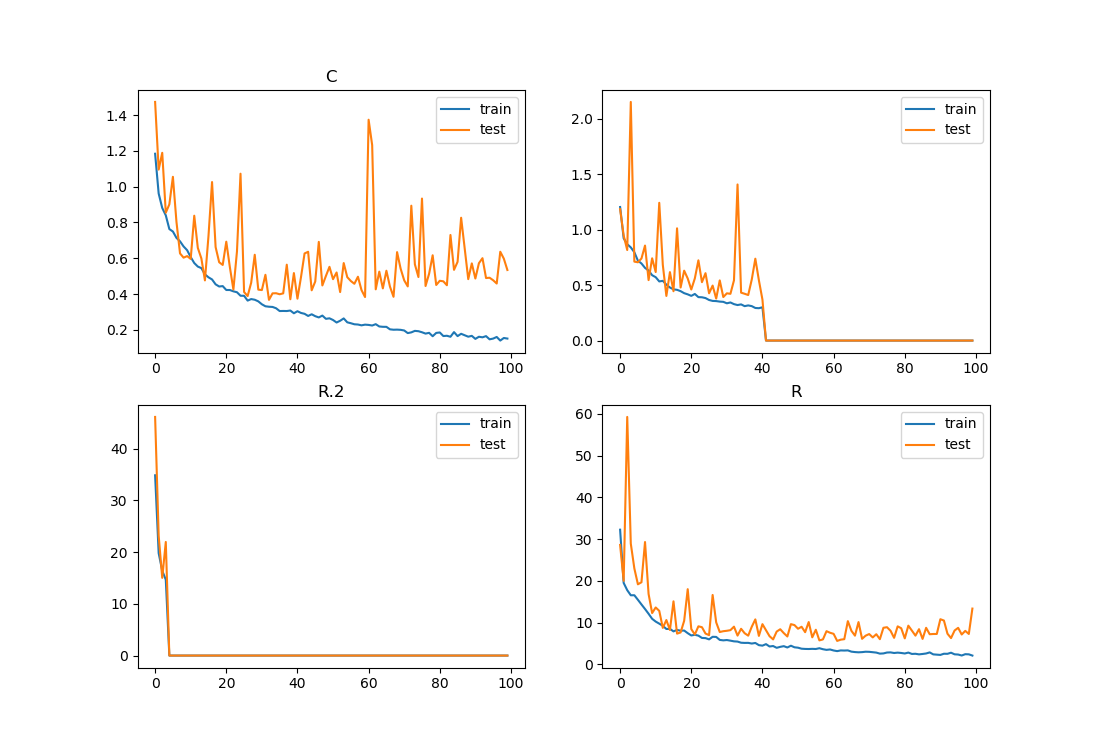
\includegraphics[width=\linewidth]{encoding_fix.results.png}
  \caption{Train and test loss results for RozNet}
  \label{fig:encoding_fix_results}
\end{figure}

\subsubsection*{Thu May 28, 2020}
After restructuring code to run with PyTorch-Lightning, I'm getting better training results. I am ommitting training-validation loss curves, since those are generated in the form of a TensorBoard log.

I also added a loss function that is calculated based on distances. Briefly, a distance matrix is calculated for each batch

\begin{equation}
\sum_{i>j} (\widehat{D}_{i,j} - D_{i,j})^2
\end{equation}
where $D_{i,j}$ is the patristic distance between the species from which sequence $i$ and $j$ come from, and $\widehat{D}_{i,j}$ is the distance between the embeddings of sequences $i$ and $j$

\begin{figure}
  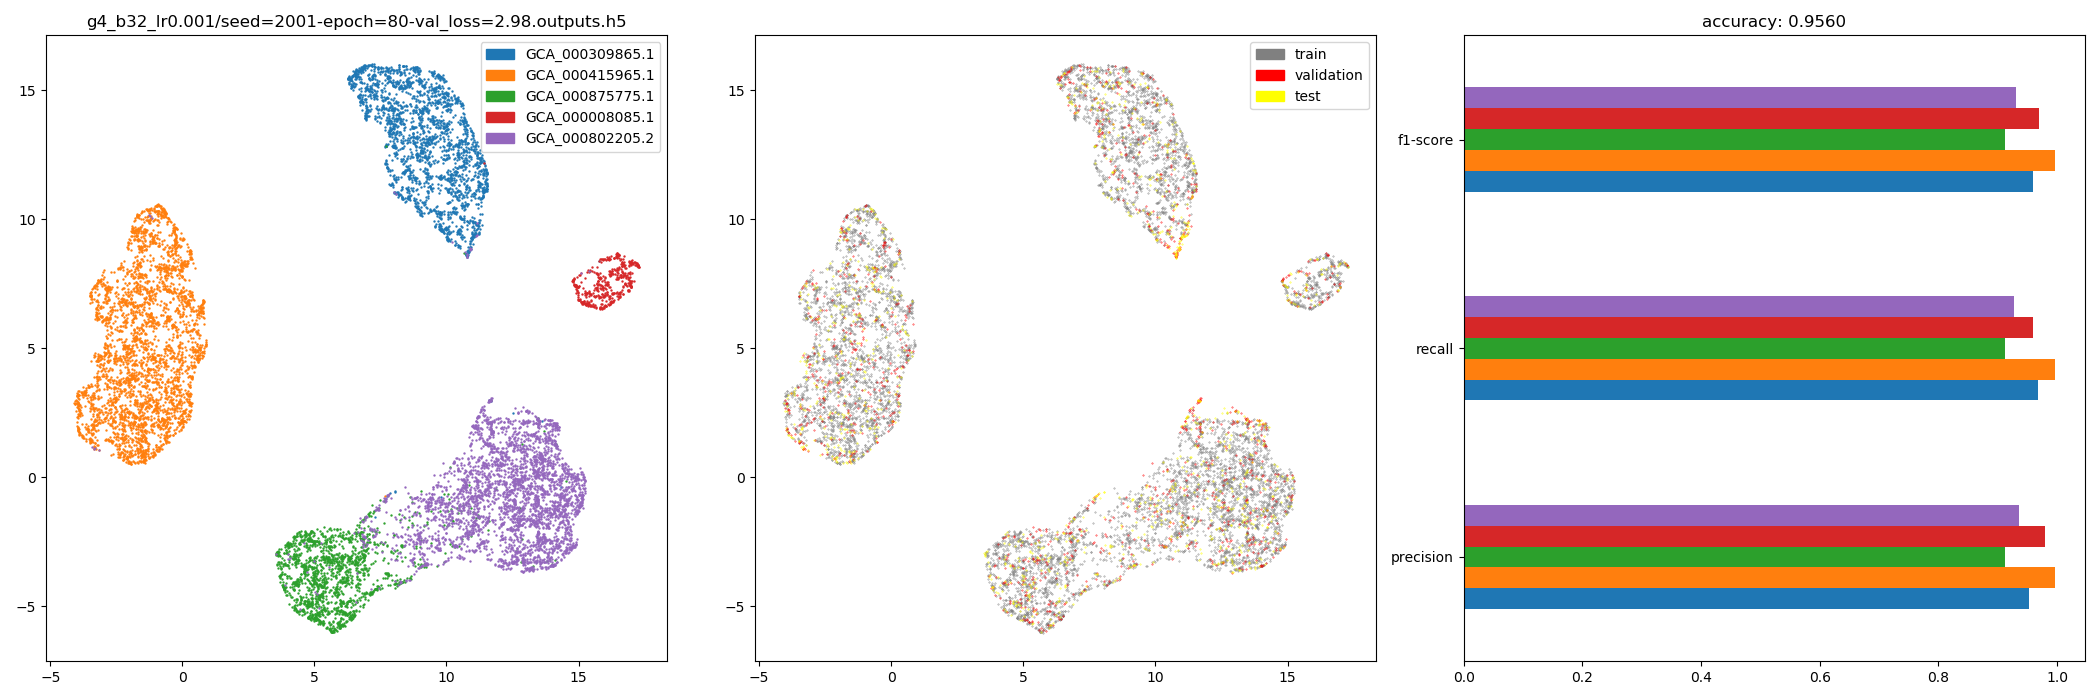
\includegraphics[width=\linewidth]{new_journal/figures/ar122_r89.genomic.small/ddp/g4_b32_lr0.001/seed=2001-epoch=80-val_loss=2.98.outputs.png}
  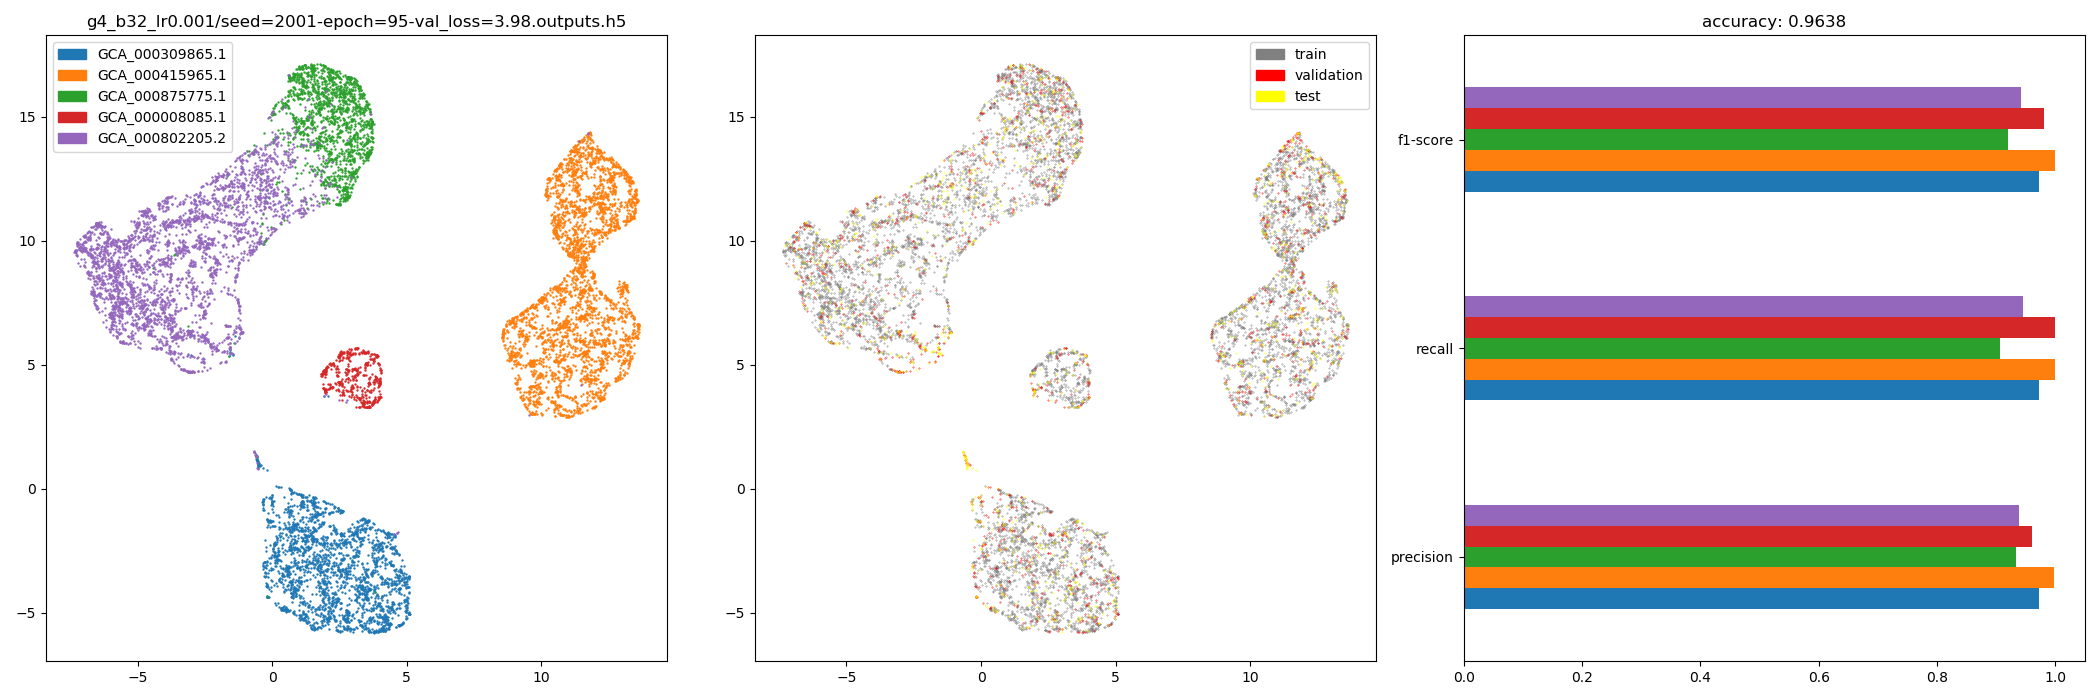
\includegraphics[width=\linewidth]{new_journal/figures/ar122_r89.genomic.small/ddp/g4_b32_lr0.001/seed=2001-epoch=95-val_loss=3.98.outputs.png}
  \caption{Final embedding results when training Roznet with distance-based loss function. Five-species archaea dataset was used.  }
  \label{fig:g4_b32_lr0.001}
\end{figure}


\subsubsection*{Tue August 18, 2020}
Since the last entry, I have moved to a bigger test dataset. This datasest uses 41 archaeal species. Within this set, I chose two species from two genera to assess
the ability to separate at the species level. I also added an embedding layer to the top of Roznet, which has speed things up substantially--I was able to run to
roughly 2000 epochs. Figure~\ref{fig:summary_roznet_medium_training} and figure~\ref{fig:summary_aggregated_roznet_medium_training} contains performance results for predicting test \emph{chunks}.
Figure~\ref{fig:summary_roznet_medium_nonrep} and figure~\ref{fig:summary_aggregated_roznet_medium_nonrep} contain performance results for predicting non-representative species.

Classification accuracy is far from perfect for all sequences, but classification accuracy is perfect for sequences above roughly 500kb.

\begin{figure}
  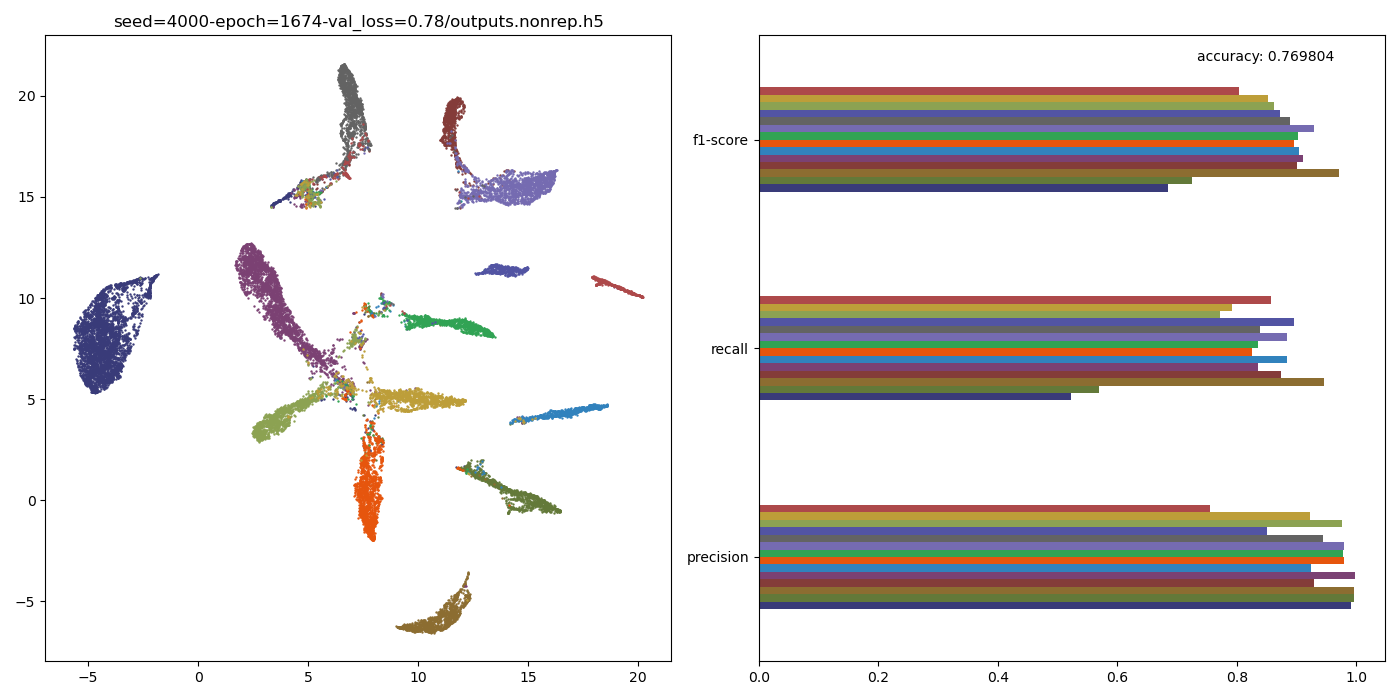
\includegraphics[width=\linewidth]{new_journal/figures/ar122_r89.genomic.medium/chunks_W4000_S4000/roznet/o256_g4_b32_lr0.001_16bit_A4/summary.png}
  \caption{Summary of chunk taxonomy prediction performance for 41-species dataset}
  \label{fig:summary_roznet_medium_training}
\end{figure}

\begin{figure}
  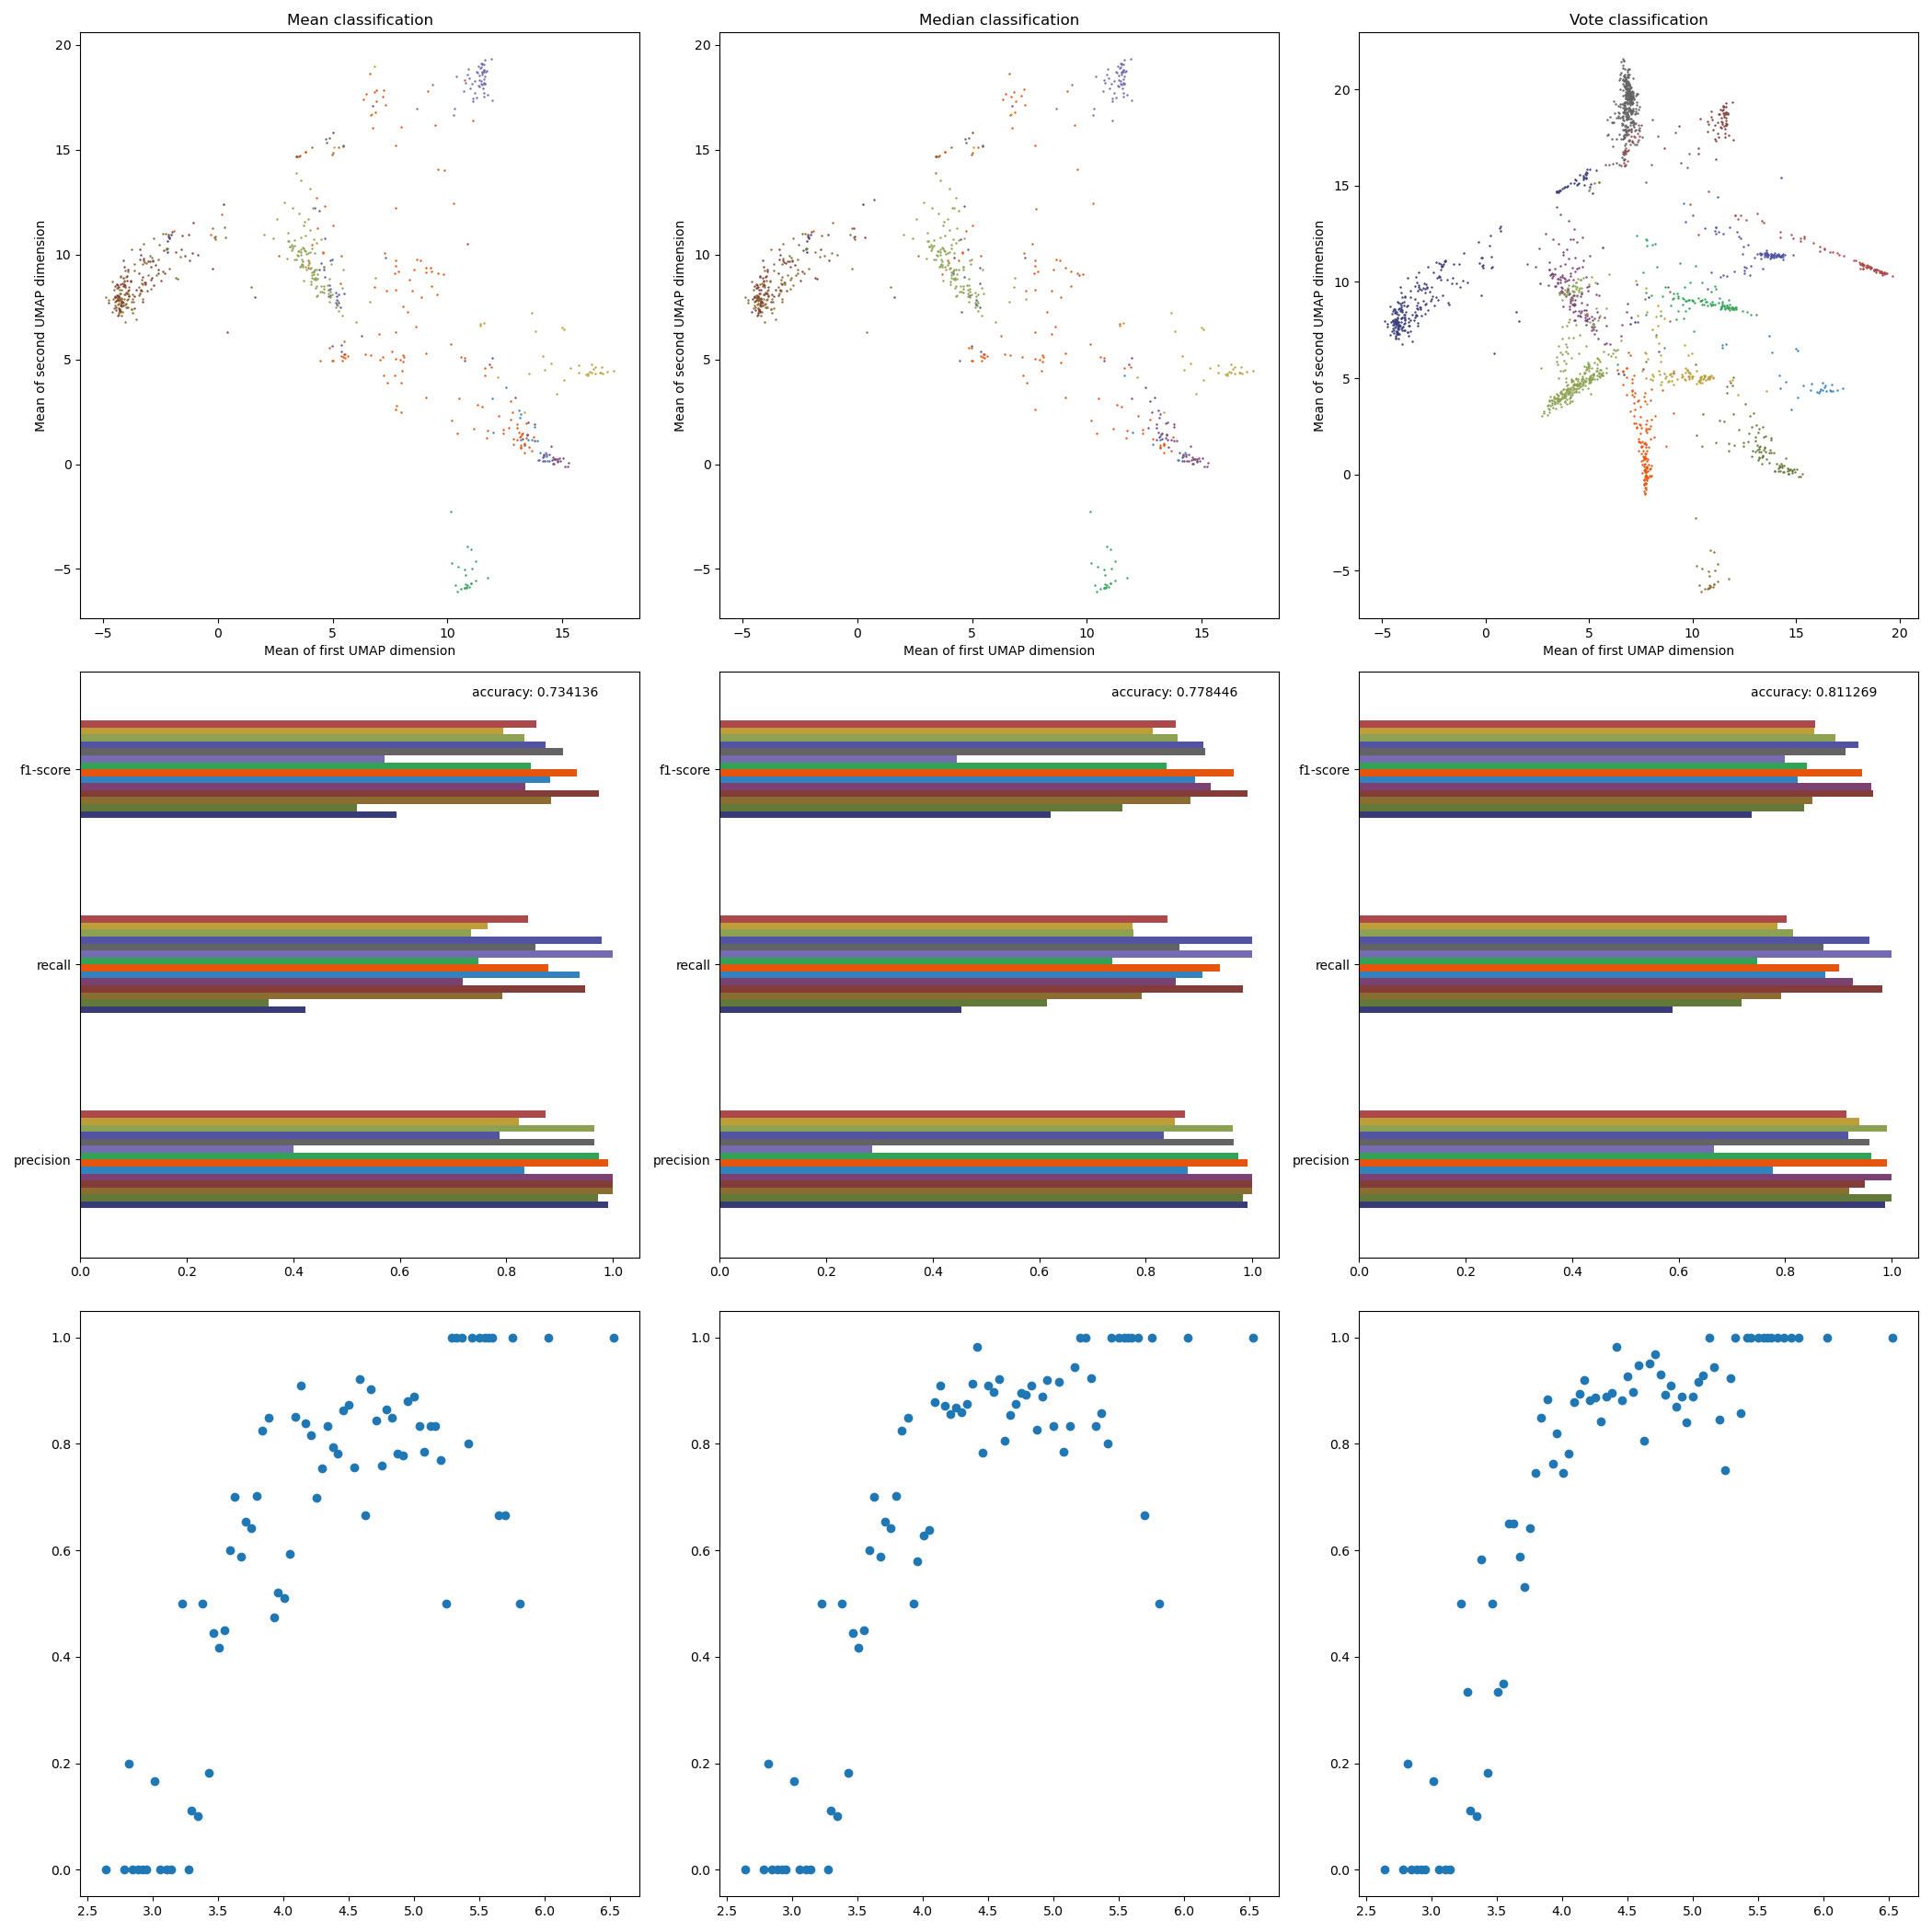
\includegraphics[width=\linewidth]{new_journal/figures/ar122_r89.genomic.medium/chunks_W4000_S4000/roznet/o256_g4_b32_lr0.001_16bit_A4/summary.aggregated.png}
  \caption{Summary of sequence taxonomy prediction performance for 41-species dataset}
  \label{fig:summary_aggregated_roznet_medium_training}
\end{figure}

\begin{figure}
  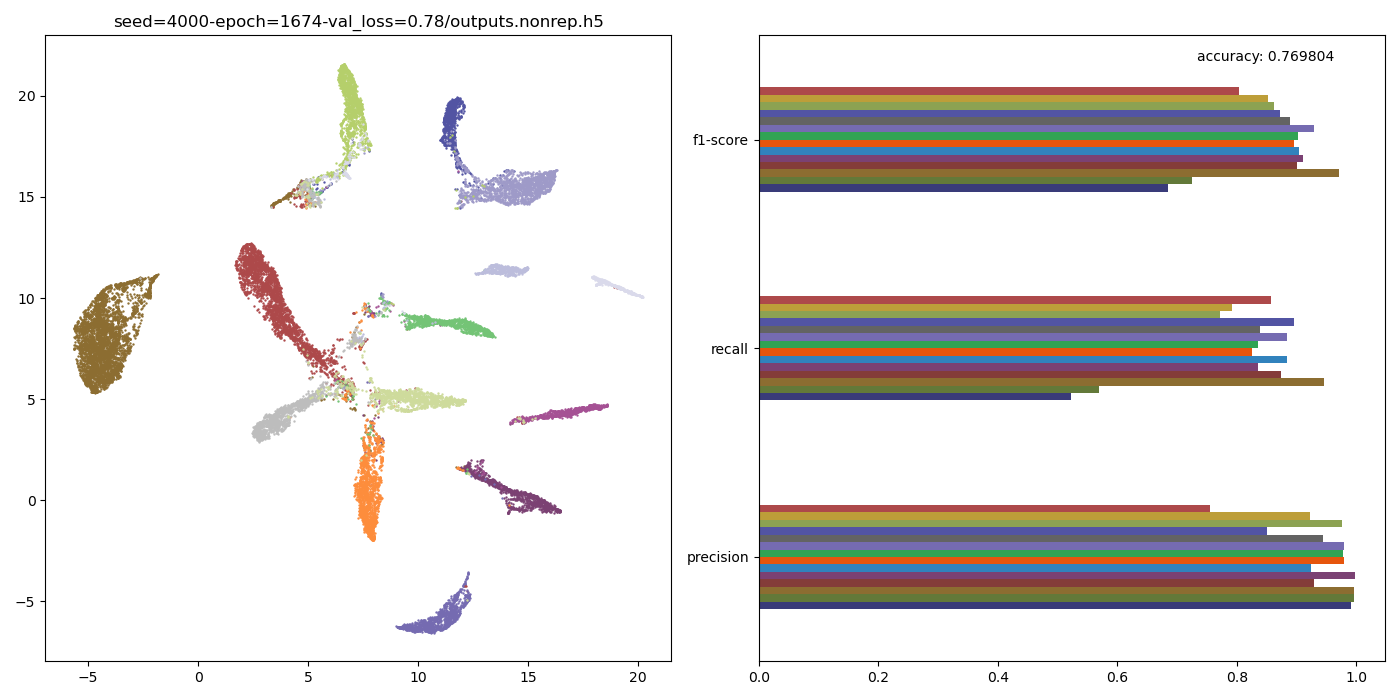
\includegraphics[width=\linewidth]{new_journal/figures/ar122_r89.genomic.medium/chunks_W4000_S4000/roznet/o256_g4_b32_lr0.001_16bit_A4/nonrep/summary.png}
  \caption{Summary of chunk taxonomy prediction performance for non-representatives of the 41-species dataset}
  \label{fig:summary_roznet_medium_nonrep}
\end{figure}

\begin{figure}
  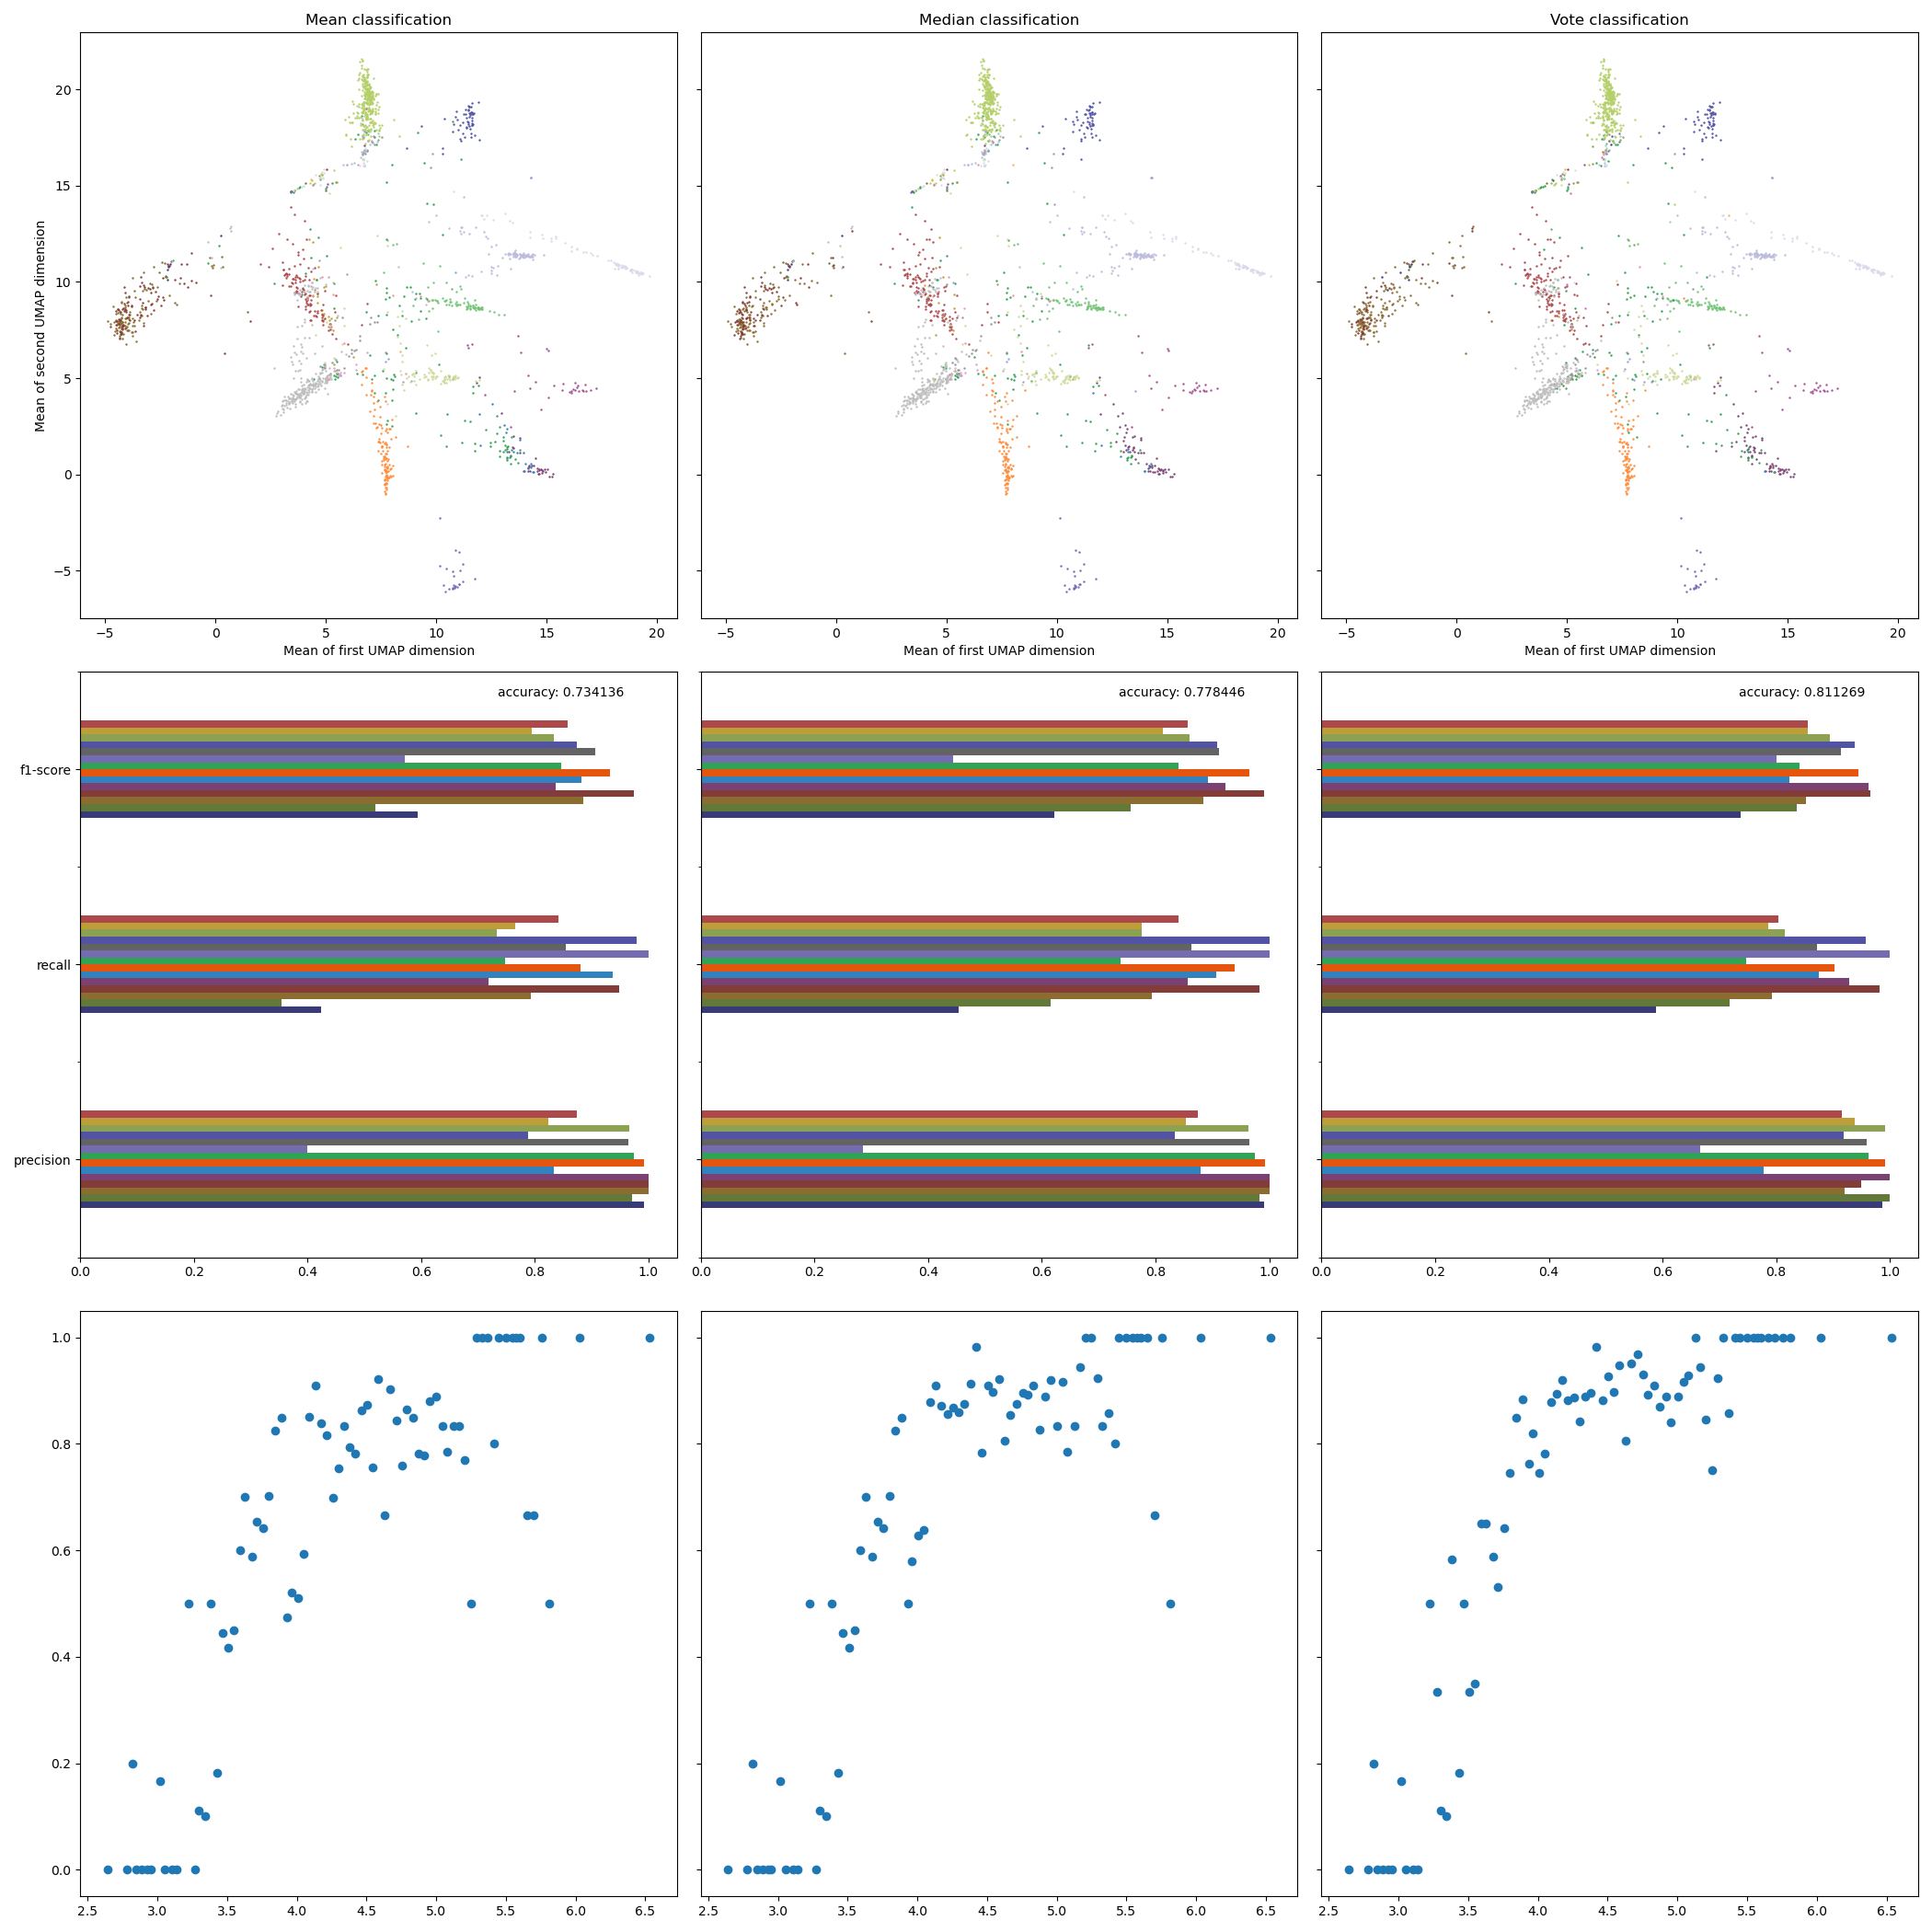
\includegraphics[width=\linewidth]{new_journal/figures/ar122_r89.genomic.medium/chunks_W4000_S4000/roznet/o256_g4_b32_lr0.001_16bit_A4/nonrep/summary.aggregated.png}
  \caption{Summary of sequence taxonomy prediction performance for non-representatives of the 41-species dataset}
  \label{fig:summary_aggregated_roznet_medium_nonrep}
\end{figure}

\end{document}

